% ---
\chapter{Fundamentação teórica}
% ---
Neste capítulo será introduzido os conceitos e fundamentos das teorias e tecnologias utilizadas neste projeto. Será abordado os paradigmas de aprendizado de máquina com foco em aprendizado por reforço. Também abordará sobre autonomia de veículos como o que define um carro autônomo e os diferentes níveis de autonomia. Por fim, o que é um motor de jogo e a principal ferramenta que usaremos para desenvolver um ambiente simulado, a Unity 3D.

\section{Veículos autônomos}
A SAE (Society of Automotive Engineers) define 6 níveis de autonomia para veículos, do zero ao cinco (\citeonline{SAE2014}). O primeiro, nível zero, não possui automação de direção alguma, é limitado a apenas a tecnologias de assistência como freios ABS ou freio automático emergencial. Um veículo com automação de nível um já passa a possuir alguns recursos que ajudam na direção, como controle para manter o carro na via, controle de velocidade a fim de manter distância de outro veículo a frente. Os níveis dois e três são definidos por, respectivamente, "direção parcialmente automática" e "direção automática condicional", a diferença de ambos pode ser bem sútil, pois em ambos os casos a automação teria o controle do volante, acelerador e freio, no primeiro seria apenas para atividades mais simples, como dirigir na estrada mantendo a velocidade e distâncias, enquanto no nível três o veículo assumiria o controle por um período, podendo até fazer manobras mais avançadas, como ultrapassar um automóvel mais lento a frente. Em ambos os níveis ainda é necessário a atenção máxima do condutor para assumir o controle quando for necessário.

Nos últimos dois níveis de autonomia, temos um veículo que seria capaz de exercer qualquer atividade sem intervenção humana, no nível 4 não seria necessário que o motorista estivesse a condução, só assumiria o controle quando necessário, nesses níveis é capaz inclusive que o automóvel assuma o controle quando necessário, e o mesmo poderia ainda nem possuir volante ou pedais.

Atualmente veículos com autonomia de nível zero a dois, já estão presentes no mercado, nesse artigo estamos interessados em discutir sobre os carros autônomos de nível 3 ou mais, isto é, automóveis que possuam um alto nível de autonomia, o sistema deles podem ser divididos em quatro componentes, cada um deles usam aprendizado de máquina de formas diferentes, são eles: planejamento de rota, decisões comportamentais, controle de moção e controle veicular. 

O planejamento de rota se trata de definir o trajeto a ser percorrido pelo veículo, isto é, o cálculo do percurso da origem ao destino, imaginar uma cidade com suas ruas, intersecções e pontos de destino como se fosse um grafo ponderado com arestas e vértices e aplicar um algoritmo de busca como Djikstra não é o suficiente para gerar uma solução eficiente, então para isso requer algo que se utilize de outros dados como informação histórica e em tempo real para achar o melhor caminho a ser percorrido em um dado dia da semana, em um dado horário e clima.

Definida a rota, o veículo deve ser capaz de percorrer a mesma tendo em consideração todos os participantes do tráfego e as regras de trânsito, isso envolve uma complexidade de comportamento que vai além de apenas saber conduzir o veículo, então o componente de decisões comportamentais deve saber selecionar ações apropriadas para cada situação. A condução do automóvel em uma rodovia é diferente da condução em um cruzamento em uma rua urbana, onde ele deve parar o veículo e cruzar quando não há nenhum outro veículo ou pedestre no caminho.

A partir do momento que o comportamento foi selecionado, o controle de moção do automóvel autônomo que decide como este vai se locomover, mudança de faixa, conversão a direita, parar o veículo, avançar ao sinal verde, etc, todos essas ações devem ser realizadas de modo que não cause colisões, evitando obstáculos, e devem de ser realizada de forma que não cause desconforto aos passageiros.

O controle do veículo se define pelo controle dos atuadores mecânicos do automóvel para que tenha uma resposta em retorno, essa constante troca de informação é necessária para o controle de moção do veículo atue apropriadamente.

\section{Motores de jogos}
Um motor de jogo (do inglês \textit{game engine}) é um \textit{software} com o objetivo primário de se criar jogos eletrônicos. Estes programas inclui diversas ferramentas que auxiliam o desenvolvedor de jogos a criar seu produto, não existe uma definição sobre quais destas um software deve possuir para ser considerado um motor de jogo, mas frequentemente possuem módulos que lidam com \textit{input} de usuário, renderização de gráficos 2D e 3D, som, motor de física (onde se lida com gravidade e colisão), animação, gerenciamento de memória entre outros (\citeonline{Andrade2015}). 

% Considerar escrever um pouco sobre outros usos de uma game engine aqui, talvez seja necessário para fortalecer o argumento que uma game engine pode ser usada para um simulador e não apenas jogos podendo ter um uso mais "sério"

Como o objetivo é focado no desenvolvimento de uma inteligência artificial para um simulador de carro autônomo, um motor de jogo possui meios que facilitariam o trabalho, não seria necessário desenvolver do zero a renderização dos modelos dos ambientes como veículos, ruas, calçadas, prédios, etc, também não seria necessário desenvolver todo o complexo cálculo de física como força, gravidade, colisão de objetos, peso do veículo, entre outros. Com isso permite que o foco do trabalho a ser feito se limite o máximo possível à análise da IA.

Inicialmente foi considerado o uso de outros motores de jogo, como a Unreal Engine 4 (software da Epic Games, Inc.) e a Godot Engine (Open Source sob licença MIT), embora haja uma preferência natural por uma ferramenta open source do que um software proprietário para realizar esta tarefa, a Unity 3D possui uma comunidade muito maior que o Godot Engine de acordo com (\citeonline{ITCHIO2023}) e (\citeonline{STEAMDB2023}), ambas as fontes são portais que servem para divulgação e venda de jogos publicados por desenvolvedores individuais ou empresas, a Unity 3D é mais utilizada em ambas as plataformas. A Unity 3D possui também seu acervo de recursos criados pela comunidade conhecido como Unity Asset Store onde é possível obter modelos 3D, efeitos sonoros e até modelos genéricos de jogos para se construir algo em cima disso. 

A Unity 3D também possui uma biblioteca de ferramentas própria para criação de agentes inteligentes chamada de \textbf{Unity ML Agent Toolkit}, que foi escrita usando \textbf{Pytorch}, uma biblioteca \textbf{Python} para criação de redes neurais. A Unity ML Agent toolkit oferece um aparato para se criar um agente inteligente, onde é configurado sensores e ações (o que seria a primeira e última camada de uma rede neural) podendo ser treinado usando aprendizado por reforço, por imitação, neuroevolução, entre outros.

\subsection{Editor da Unity3D}
Dentre as principais janelas da interface da Unity3D, temos: hierarquia, projeto, visualização da cena e inspetor. A primeira se trata dos elementos que há dentro da cena (pode-se entender como sendo um trecho do jogo, como este projeto contém apenas uma única cena não é necessário que o leitor entenda tudo que uma cena pode ser), estes elementos são chamados de \textit{GameObjects}, eles são uma abstração de qualquer item dentro do jogo, incluindo o personagem que o jogador controla, o cenário com o qual interage, a "câmera" com o qual o jogo é visto também é um \textit{GameObject}. A primeira janela é chamada de hierarquia porque o conjunto destes objetos podem formar uma estrutura em árvore, por exemplo, podemos criar um objeto "árvore" que conteria os objetos "raiz", "tronco" e "folhas" como seus objetos aninhados. Na seção da proposta é explicado a estrutura deste projeto com mais detalhes.

\begin{figure}[h]
   \centering
   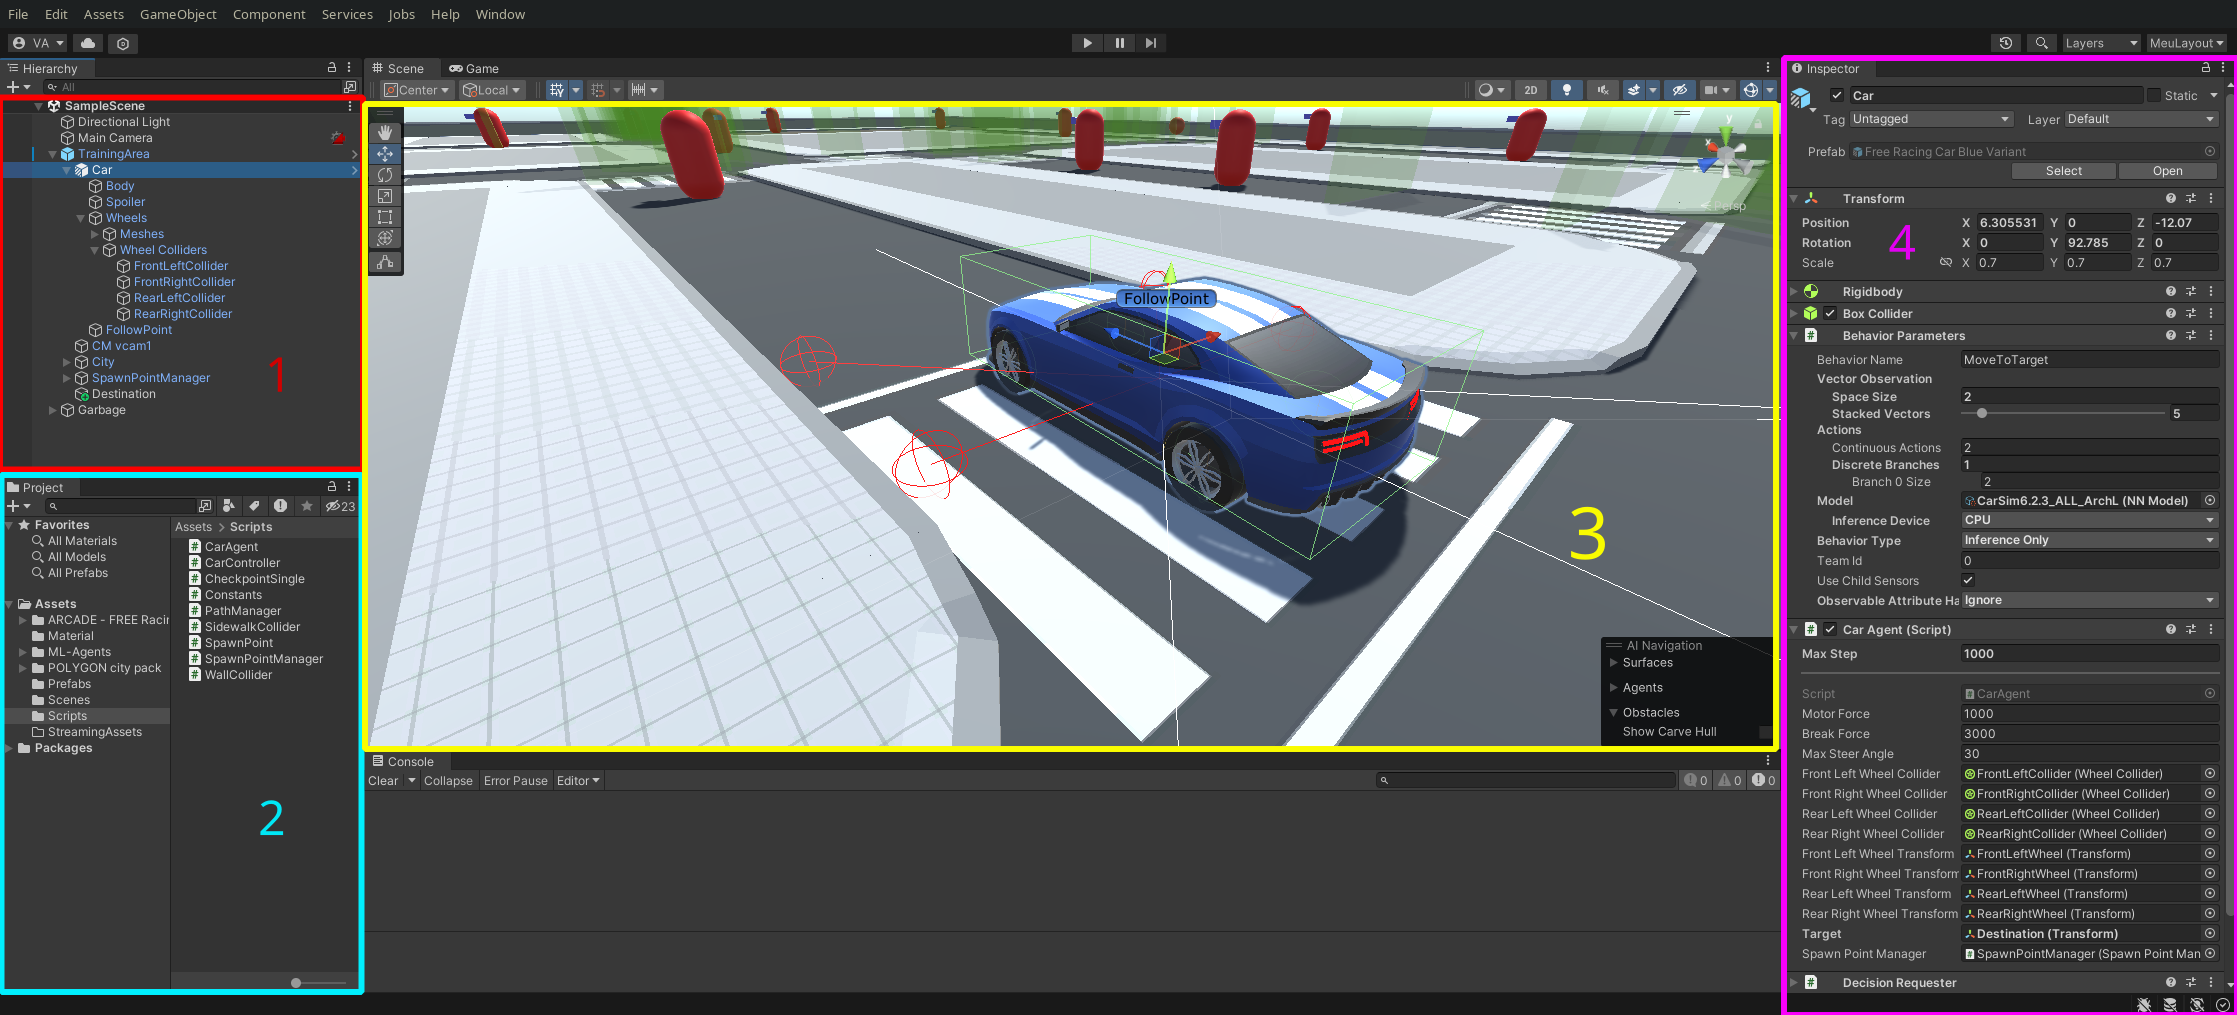
\includegraphics[scale=0.2]{figs/interface-unity3d-indicadores.png}
    \caption{Interface da Unity3D. A janela 1 é a hierarquia, 2 é a janela de projeto, 3 é visualização da cena e 4 é o inspetor}
    \label{fig:prefixt}
 \end{figure}

A janela de projeto estão os arquivos do projeto, é um diretório do projeto criado pela Unity3D onde deve conter arquivos de efeitos sonoros, códigos-fonte do desenvolvedor, fontes, modelos 2D e 3D, texturas, etc. A visualização da cena é uma janela que permite o desenvolvedor ter uma noção visual da disposição dos \textit{GameObjects}, desta forma ele consegue posicioná-los mais apropriadamente, também consegue ver se a dimensão e escala deles estão coerentes. 

A última janela é o inspetor, nela é exibido os detalhes dos \textit{GameObjects}, isto é, os \textit{components} destes. Como foi explicado anteriormente, os \textit{GameObjects} podem assumir diversas funcionalidades, e são os componentes que permitem isso, por exemplo, o componente \textit{Transform}, comum a todos os objetos da cena define as coordenadas (ou posição) que o objeto se encontrará na cena, sua rotação e escala, já os \textit{components} \textit{Mesh Filter} e \textit{Mesh Renderer} são responsáveis pela renderização 3D de um objeto, isto é, sua forma e aparência.

Os conceitos de como funciona um desenvolvimento de jogo dentro do editor da Unity3D podem não ter ficado claro ao leitor, porém na parte sobre o sistema proposto deste artigo é explicado em mais detalhes a estrutura do projeto.

\section{Inteligência Artificial}
Não existe uma definição única sobre o que é Inteligência Artificial (IA), o mesmo pode ser dito quanto ao seu objetivo. Porém, para compreender melhor o seu escopo, pode-se dizer que está interessada em criar um programa de computador que faça uma ou mais dos seguintes tópicos: pensar humanamente, agir humanamente, pensar racionalmente e agir racionalmente. Pensar pode ser entendido como o processo de pensamento, de compreender e argumentar enquanto agir pode ser entendido como tomar ações e possuir um certo comportamento. Humanamente mediria o quanto a Inteligência Artificial consegue se aproximar de um desempenho humano (agindo ou pensando), e racionalmente é quando há o interesse em pensar ou agir de forma ideal, isto é, que faça "a coisa certa" (\citeonline{Russell2009-dn}).

Uma IA que age racionalmente, pode ser entendido como um programa de computador que toma decisões autonomamente. De fato, qualquer algoritmo pode ser criado para tomar decisões de acordo com uma série de condições, mas é esperado mais de um \textbf{agente racional}, ele é criado para observar o ambiente em que está inserido e tomar decisões por um período prolongado, adaptando-se a qualquer mudança e procurando cumprir seu \textbf{objetivo} fazendo isso de forma ideal, não cometendo erros, e quando estes forem inevitáveis, deverá agir de forma a minimizar o dano causado (\citeonline{Russell2009-dn}).

Para desenvolvimento de um veículo autônomo que este artigo se propõe a estudar, não basta um algoritmo definindo condições e instruções, isto seria uma abordagem insuficiente tanto em eficiência quanto em praticidade em seu desenvolvimento. Seria então necessário uma agente racional, que possua as características descritas no parágrafo anterior, que saiba observar o ambiente em sua volta e \textbf{aprenda} a agir de acordo. A seção abaixo elabora mais sobre esta área específica da Inteligência Artificial.

%-
\subsection{Aprendizado de máquina}
%-
Aprendizado de máquina é qualquer processo automatizado que tem como objetivo reconhecer um padrão dentro de um conjunto de dados (\citeonline{Kelleher2015-iw}), em aprendizado de máquina o projetista cria um agente-aprendiz, fornece os dados e define um objetivo a fim de fazer seu agente melhorar seu desempenho na tarefa após sucessivas iterações observando os dados o tomando decisões. 

Há dois paradigmas em AM que valem a pena ser mencionados brevemente antes de irmos ao que será utilizado no projeto, são eles: Aprendizado supervisionado, não-supervisionado. O primeiro lida mais com problemas de classificação, ao agente é fornecido dados rotulados, e ao analisá-los, se o treino foi efetivo, o agente seria capaz de atribuir um rótulo a um novo registro com uma alta acurácia. O Aprendizado não-supervisionado envolve dados sem rótulos, o objetivo do agente é encontrar uma estrutura oculta que conecte os dados, este processo é chamado de clusterização. Embora possa haver espaço para estes paradigmas no campo de autonomia veicular, eles não estão no escopo deste projeto.

% ---
\section{Aprendizado por reforço}
% ---
No aprendizado por reforço o objetivo é sempre fazer com que o agente aprenda a executar uma tarefa, se trata de ensiná-lo a como fazer. O agente está inserido em um ambiente e a ele é dado um objetivo, com isso ele deve aprender a tomar as decisões corretas nas situações apropriadas visando seu propósito. O aprendiz não é instruído sobre quais ações tomar em dadas circunstâncias, ao invés disso o agente aprenderá a tomar as decisões com base na orientação do treinamento, que envolve em premia-lo quando agir idealmente ou penaliza-lo caso contrário. Esse parecer que o agente recebe é um valor numérico a ser maximizado por ele, e o dever do projetista é programar os critérios que decidem não somente o que é recompensador ou penalizador, mas o quanto é.

\subsection{Elementos do Aprendizado por Reforço}
Além do agente-aprendiz que há em outras formas de aprendizado mencionadas anteriormente, este paradigma possui outros elementos principais que devem ser identificados quando tenta-se resolver qualquer problema utilizando aprendizado por reforço. Nesta seção cobrirá em mais detalhes os seguintes componentes: a \textbf{política}, o \textbf{sinal de recompensa} e a \textbf{função valor}.

\begin{figure}[h]
   \centering
   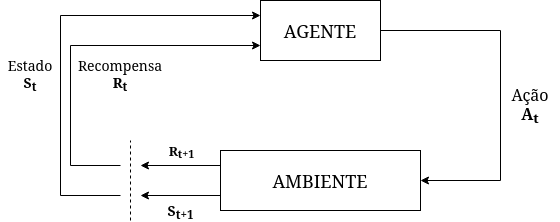
\includegraphics[scale=0.75]{figs/RL-diagram.drawio.png}
    \caption{diagrama da interação do agente com o ambiente. Adaptado de \citeonline{rl-sutton-barto}}
    \label{fig:prefixt}
 \end{figure}

A \textit{política} é o mapeamento do estado percebido do ambiente em ações a serem tomadas naquele estado, é a fórmula que determina qual a decisão correta dadas as observações do ambiente. A política pode ser estocástica, especificando probabilidades para cada ação, algumas maiores que outras.

A recompensa é o número a ser maximizado pelo agente aprendiz, ele indica se o mesmo cumpriu ou está se comportando como deveria. A cada passo, o agente ajusta suas ações com base no sinal de recompensa recebido, se o mesmo é positivo ele deve entender que as ações que tomou foram apropriadas, caso contrário deve buscar mudar seu comportamento a fim de buscar recompensas maiores. Punir em excesso o agente por cometer erros, na intenção de ter um treino mais rigoroso, pode acabar deixando-o sem orientação do que fazer, por outro lado, recompensá-lo demasiadamente pode fazê-lo com que aja inapropriadamente sem se atentar às consequências.

O valor de um estado no ambiente é o tanto de recompensa que o agente espera ganhar no futuro partindo daquele estado. Se o sinal de recompensa indica o que é bom em curto prazo, o valor do estado indica o quanto o agente pode ganhar no longo prazo, talvez \textit{vale} mais a ele ganhar uma recompensa menor se no longo prazo ele receber um montante maior. Recompensas são o objetivo primário, enquanto valores, que são predições de recompensas futuras, são secundários. Se não há recompensas não haverá valores, porém é este último que requer mais atenção de um pesquisador treinando um agente via aprendizado por reforço. Enquanto que recompensas são fáceis de definir, pois basta punir quando algo indesejado ocorrer e premiar caso contrário, maximizar o valor é mais complexo, o agente pode criar o vício de fazer o errado para ganhar recompensas maiores. E é de interesse do aprendizado que o agente tome decisões que leve a maiores valores e não maiores recompensas.

\subsection{Algoritmos de otimização de política}
Nesta seção será abordado mais sobre os diferentes tipos de algoritmos de otimização de política, principalmente o PPO, SAC que estão disponíveis no ML-Agents da Unity 3D.